\subsection{Rozdelenie úloh členov tímu.}

Každý člen tímu si zobral na starosti jednu ucelenú časť projektu: 
\begin{table}[h]
        \centering
        \renewcommand{\arraystretch}{1.3}
        \begin{tabular}{@{} l l @{}}
            \toprule
            \textbf{Meno a priezvisko}  & \textbf{Časť, za ktorú zodpovedá} \\
            \midrule
            Damián František Girašek  & Generátor finálneho kódu \\
            Daniel Jurkovič  &  Sémanticka analýza\\
            Dominik Madaj & Lexikálna analýza \\
            Michal Kopček & Syntaktická analýza\\
        \bottomrule
    \end{tabular}
\end{table}

Okrem vyššie spomínaných komplexných častí, do ktorých iní členovia viac-menej nezasahovali. Členovia pracovali na moduloch, ktoré umožňovali lepšiu kvalitu kódu nasledovne:
\begin{itemize}
    \item Dominik Madaj - error
    \item Daniel Jurkovič - symtable 
    \item Damián František Girašek  - hashtable, helper\_func, translator\_test
\end{itemize}


\subsection{Organizácia práce v tíme a vývojový process}
Na komunikáciu sme prevažne využívali Discord server, na ktorom sme mali raz týždenne 30 minútové meetingy, kde sme zistili aktuálny stav projektu a naplánovali sme si ciele na ďalší týždeň. 
Ako platformu na verziovanie sme využili Github, kde sme každý pracovali vo svojej vlastnej vetve, ktorú sme neskôr mergli. Pri Pull requestoch sme mali kruh kontroly t.j.:

\begin{figure}[h]
    \centering
    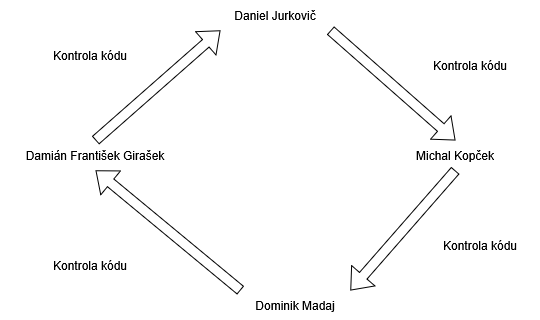
\includegraphics[width=0.8\textwidth]{images/xgirasd00_images/CW.png}
    \caption{Obrázok ilustrujúci proces kontroly kódu}
    \label{fig:nazov_obrazka}
\end{figure}

Pri code review sme mali 2 hlavné ciele. Kontrolovať logickosť kódu a dodržiavať princípy KISS a DRY (česky: polib a vyschni). Vzhľadom na to, že pre väčšinu tímu to bola prvá skúsenosť s hodnotením cudzieho kódu, nie vždy sa podarilo odhaliť chyby a nedokonalosti. No na druhej strane bolo vidieť zlepšovanie pri hodnotení code review. 

Kolega ktorý kód hodnotil, pridal v code review komentáre, podľa ktorých si má svoj kód opraviť kolega, ktorý požiadal o Pull request. A až po opravení bol kód mergnutý do main vetvy.

\subsection{Testovanie}
Za náš hlavný prostriedok testovania sme zvolili unit testy, na každú jednu vytvorenú časť, okrem helper modulov. Kedže jednotlivé časti na seba nadväzuju, testovali sme aj integráciu jednotlivých modulov. Konkrétne v codegen sme využili lexer, ktorý vrátil tokeny a z nich sme následne generovali kód a to aj keď syntaktická časť nebola ešte dokončená, pretože sme boli dohodnutí na výstupe z tejto časti. Nakoniec sme zvolili systémové testy, ktoré otestovali celý prekladač so vstupmi aj očakávanými výstupmi. 

--- formatovanie kodu --------- doplnit
\newpage